
\section{Đọc trade-off, ma trận lỗi và độ ổn định}
Phần này hoàn tất bộ hình dự kiến từ prediction đã khóa. Hai target 1\%/5\% do validation quyết định; trục FPR trong hình trade-off là FPR quan sát trên test. Mean/sample std dùng năm seed trên cùng official test, không phải khoảng tin cậy hoặc bằng chứng tổng quát ra hệ thống vận hành. CS không có held-out nên không vẽ UADR CS. Ma trận dùng seed 42 đã định trước, không chọn seed có kết quả đẹp.

\begin{figure}[H]\centering
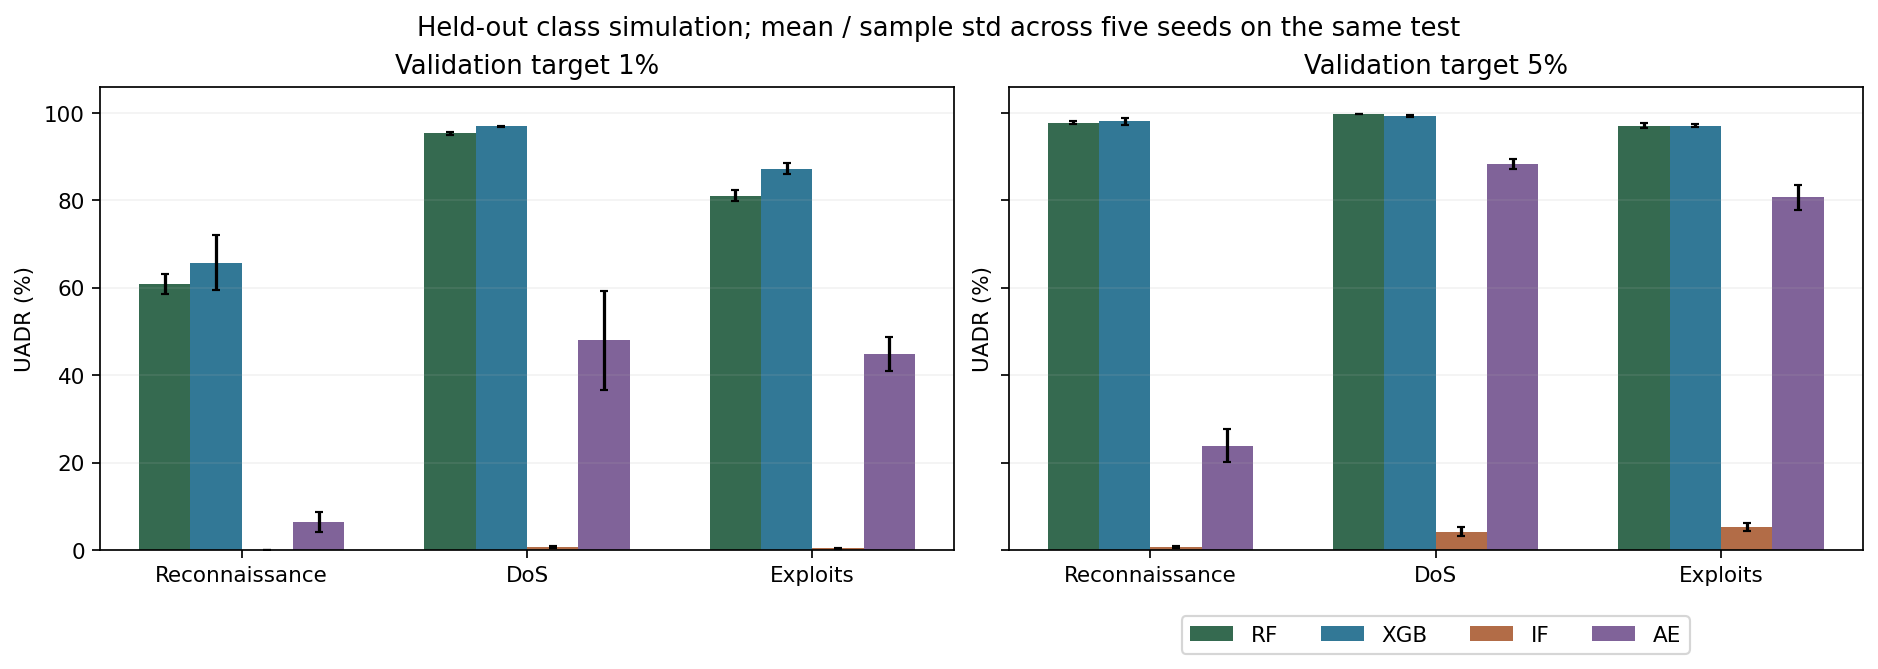
\includegraphics[width=.98\textwidth]{assets/final_diagnostics/UADR_BOTH_TARGETS.png}
\caption[UADR tại hai target validation]{UADR theo ba lớp held-out ở hai target validation; mean/sample std qua năm seed, mô phỏng giấu lớp.}\end{figure}

\begin{figure}[H]\centering
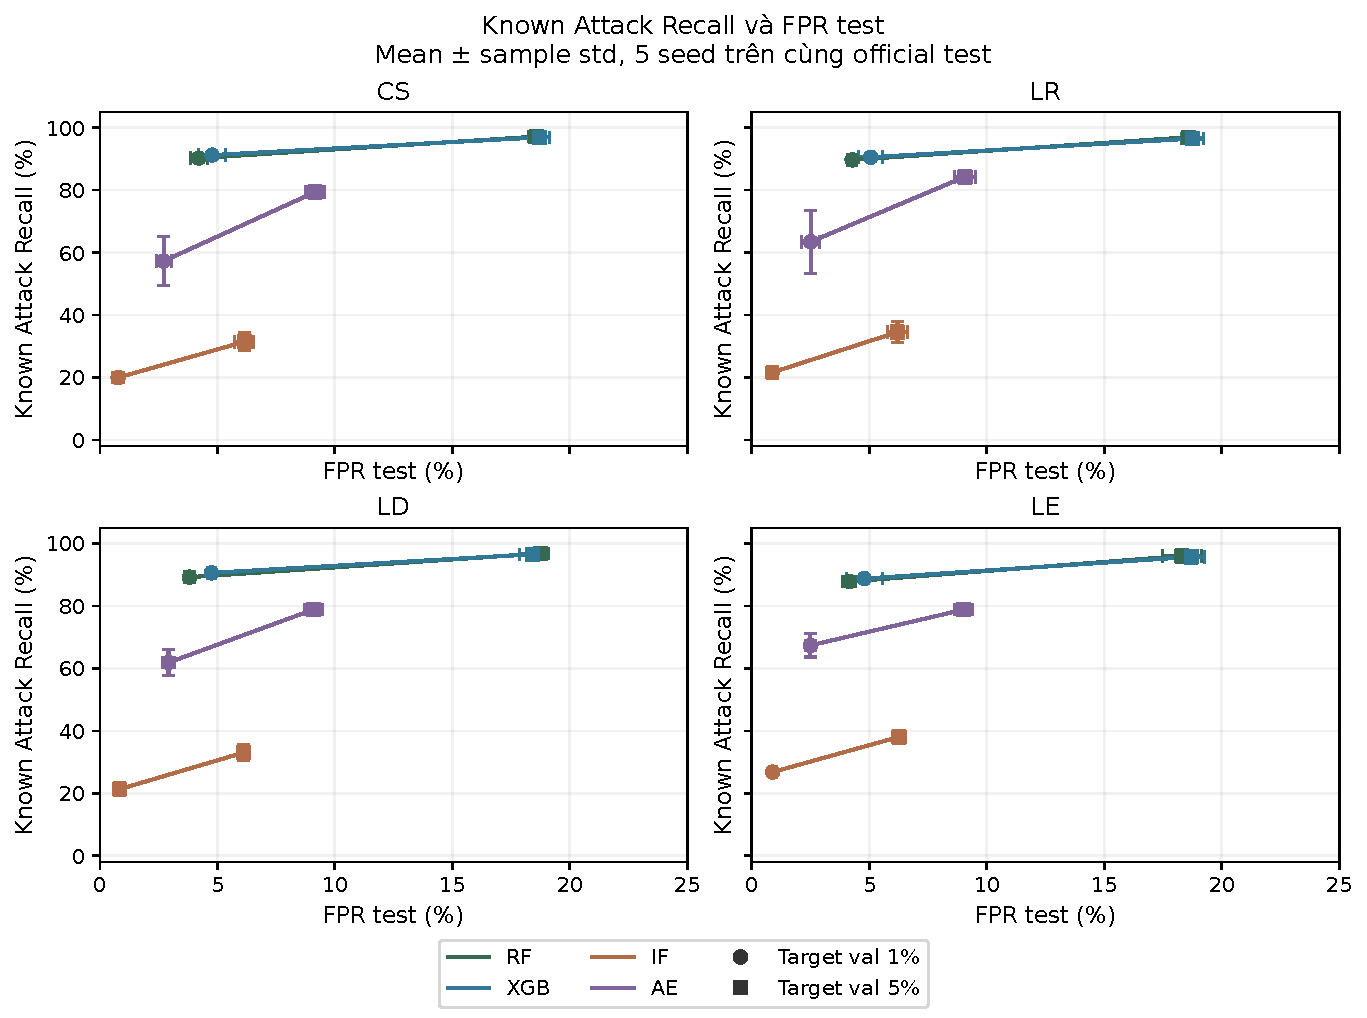
\includegraphics[width=.98\textwidth]{assets/final_diagnostics/TRADEOFF_KNOWN_RECALL.pdf}
\caption[Known Attack Recall theo FPR test]{Known Attack Recall theo FPR test quan sát; hai điểm là target validation 1\%/5\%, mean/sample std năm seed.}\end{figure}

\begin{figure}[H]\centering
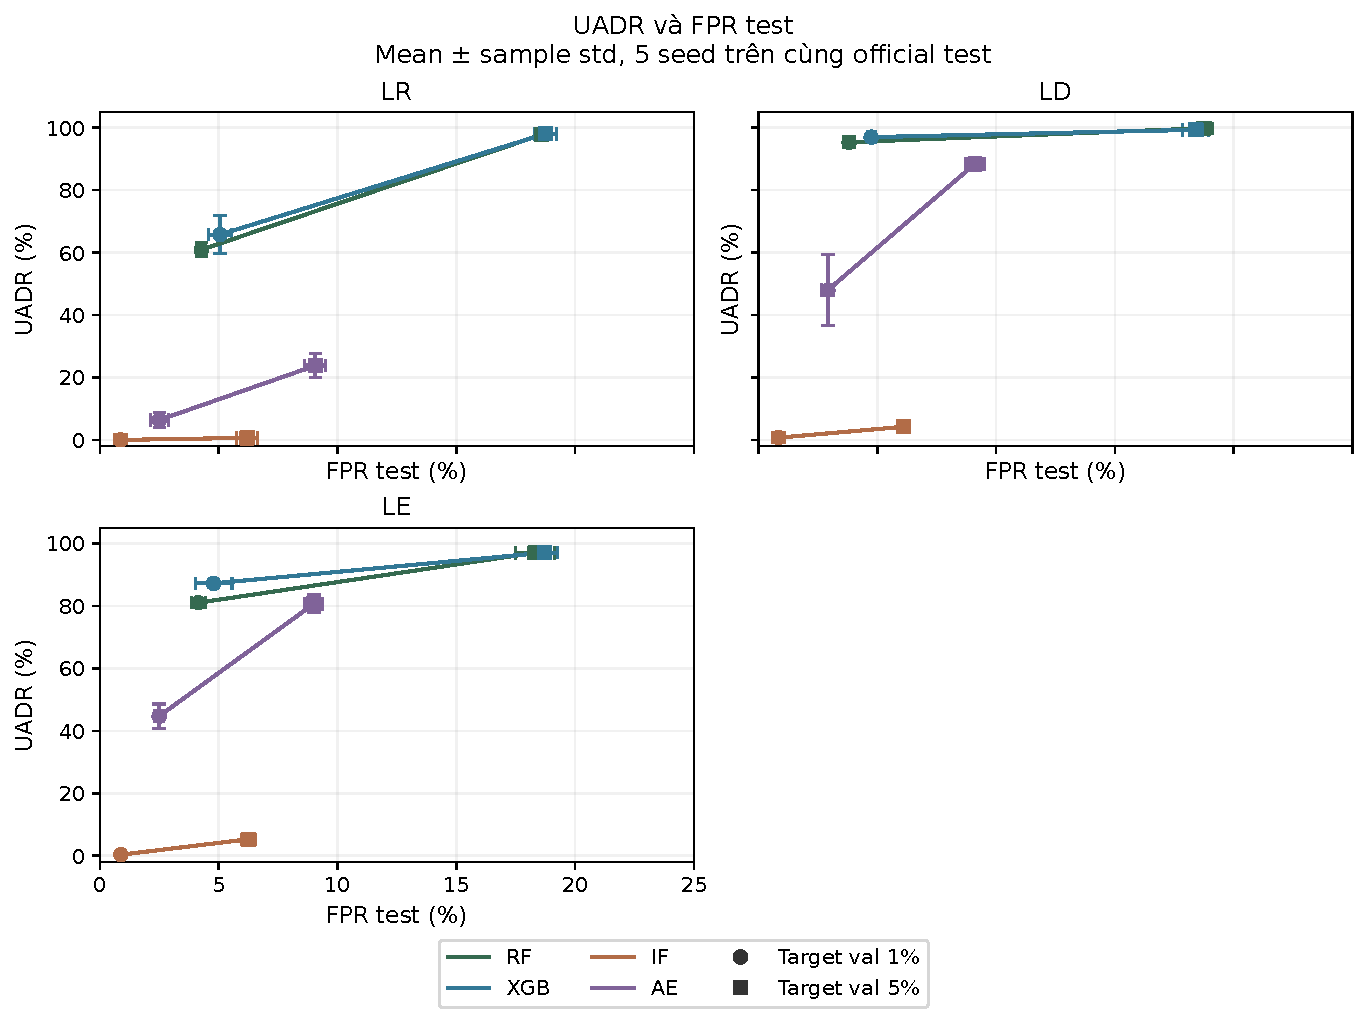
\includegraphics[width=.98\textwidth]{assets/final_diagnostics/TRADEOFF_UADR.pdf}
\caption[UADR theo FPR test]{UADR theo FPR test quan sát; ba LOACO, mean/sample std năm seed. Đọc đồng thời khả năng bắt held-out và báo nhầm.}\end{figure}

\begin{figure}[H]\centering
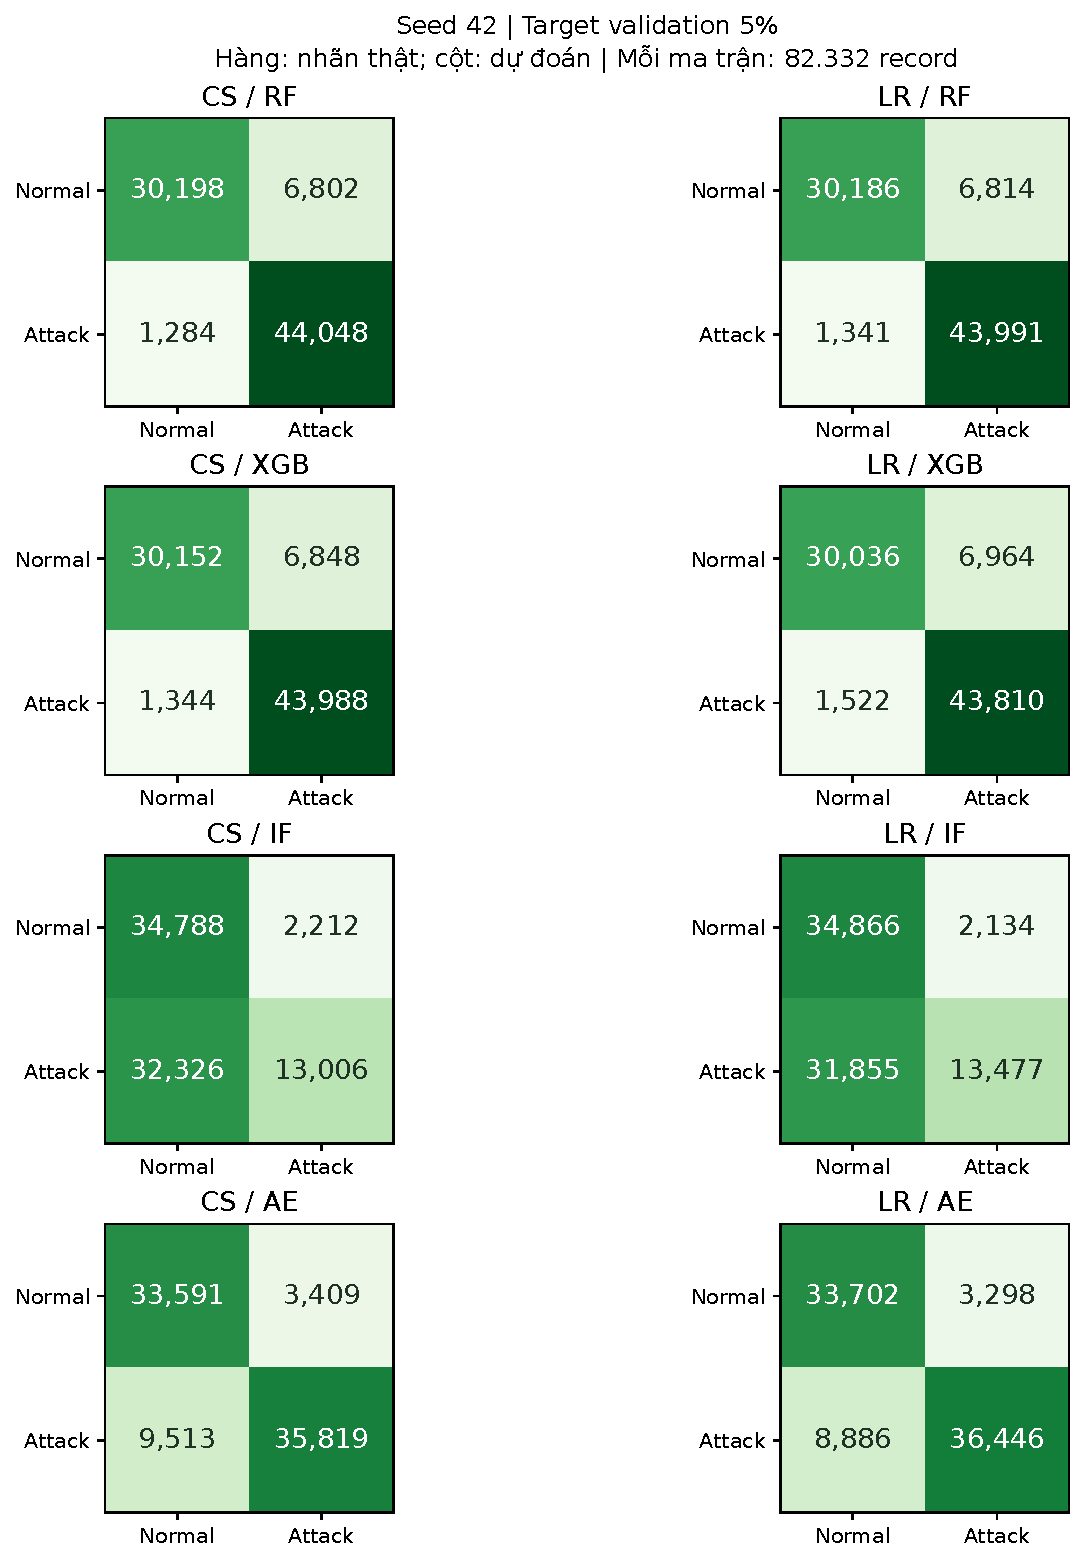
\includegraphics[width=.96\textwidth]{assets/final_diagnostics/CONFUSION_CS_LR_S42.pdf}
\caption[Ma trận nhầm lẫn CS và LR]{Ma trận nhầm lẫn CS và LOACO Reconnaissance; bốn model, seed 42, target validation 5\%. Hàng là nhãn thật; cột là dự đoán.}\end{figure}

\begin{figure}[H]\centering
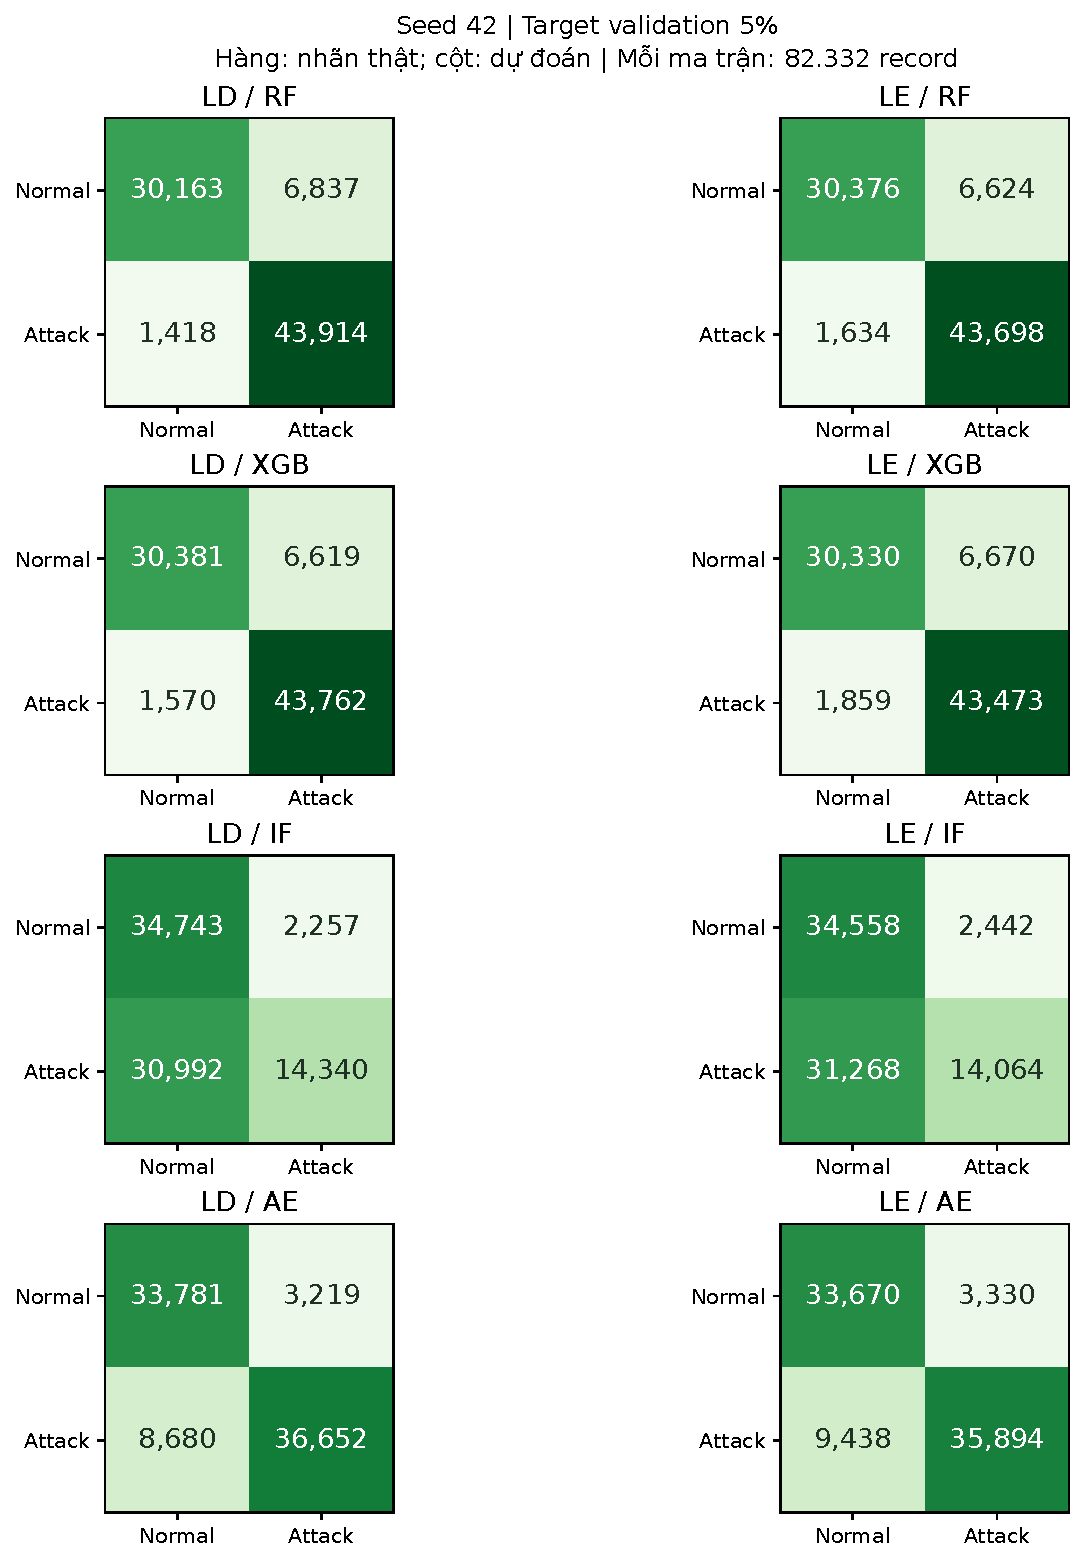
\includegraphics[width=.96\textwidth]{assets/final_diagnostics/CONFUSION_LD_LE_S42.pdf}
\caption[Ma trận nhầm lẫn LD và LE]{Ma trận nhầm lẫn LOACO DoS và Exploits; bốn model, seed 42, target validation 5\%. Hàng là nhãn thật; cột là dự đoán.}\end{figure}

\begin{figure}[H]\centering
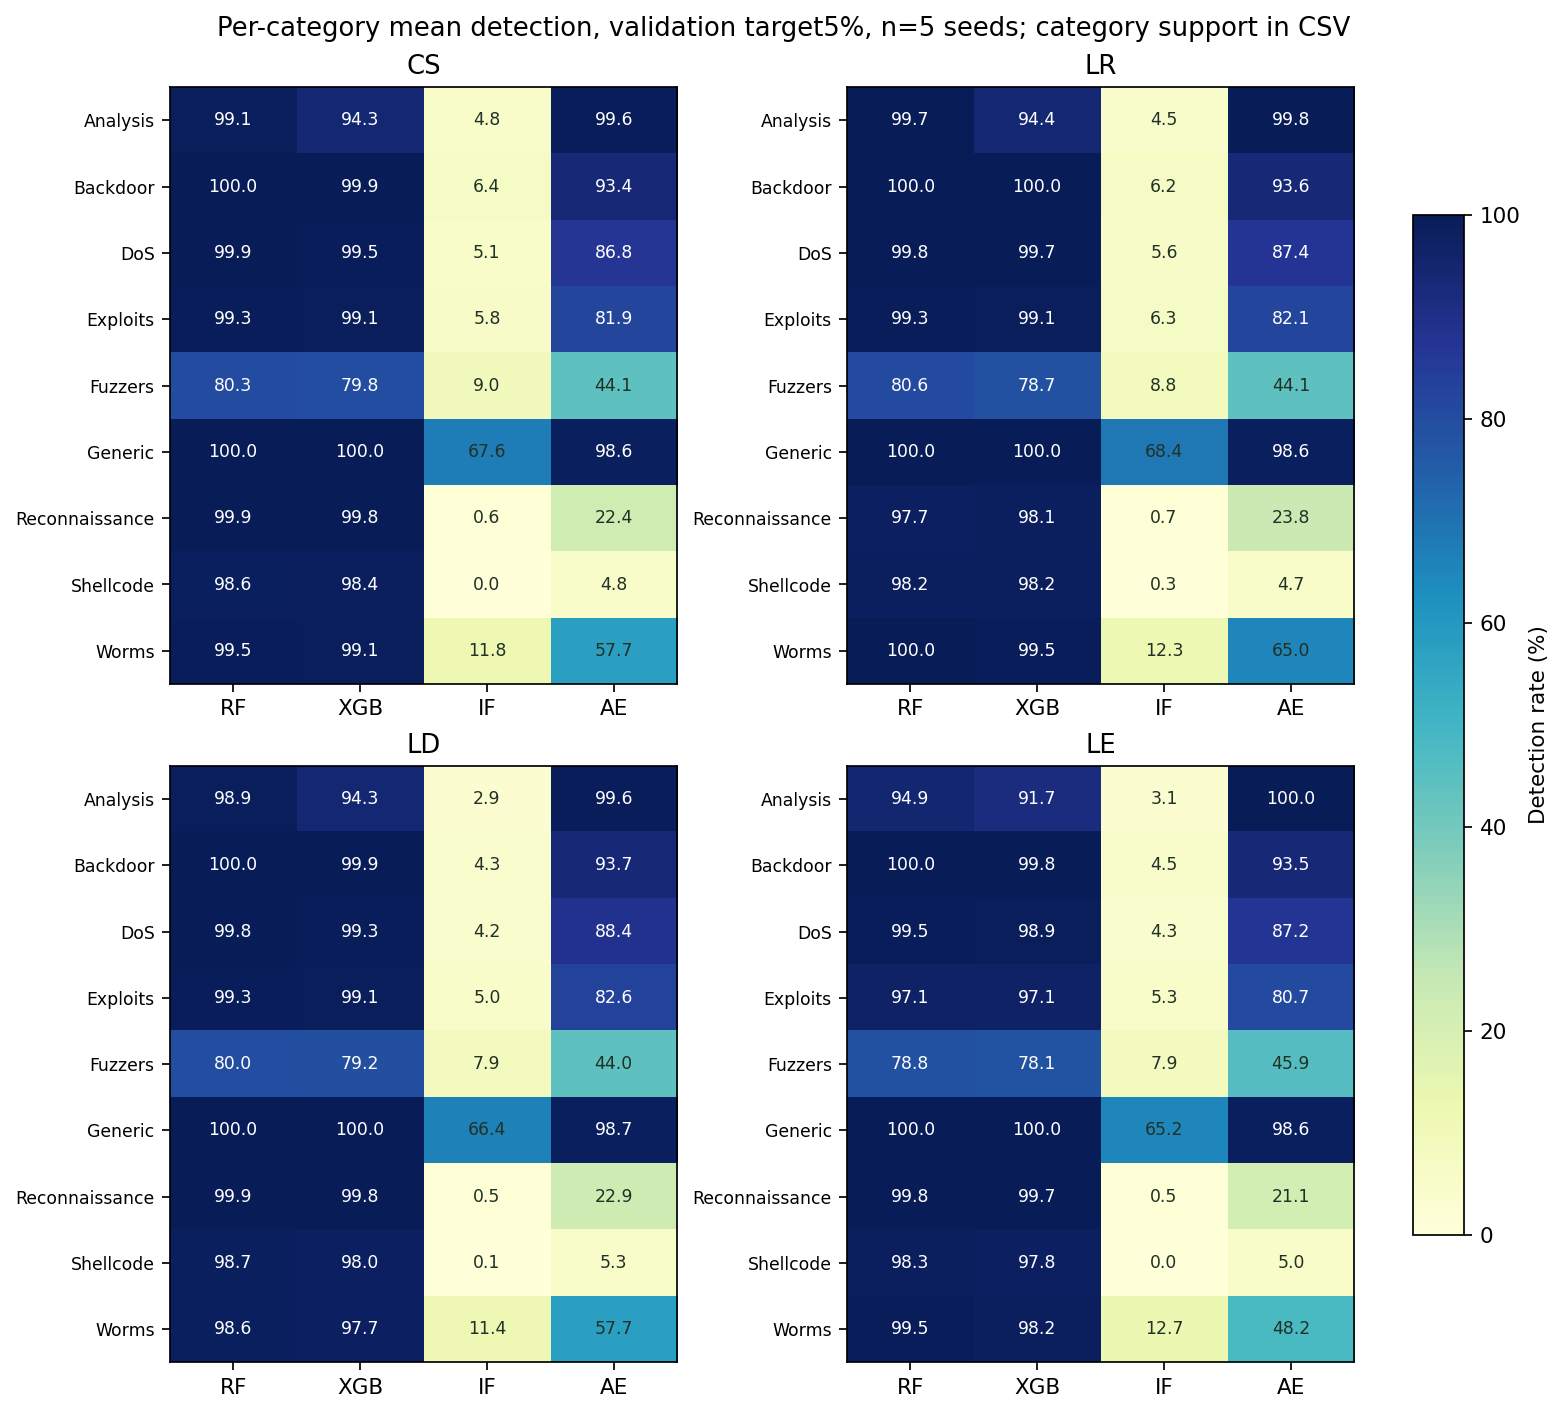
\includegraphics[width=.94\textwidth]{assets/final_diagnostics/CATEGORY_DETECTION_HEATMAP.png}
\caption[Detection rate theo attack category]{Detection rate từng attack category, target validation 5\%; mean năm seed; support đầy đủ trong CSV category.}\end{figure}

\begin{figure}[H]\centering
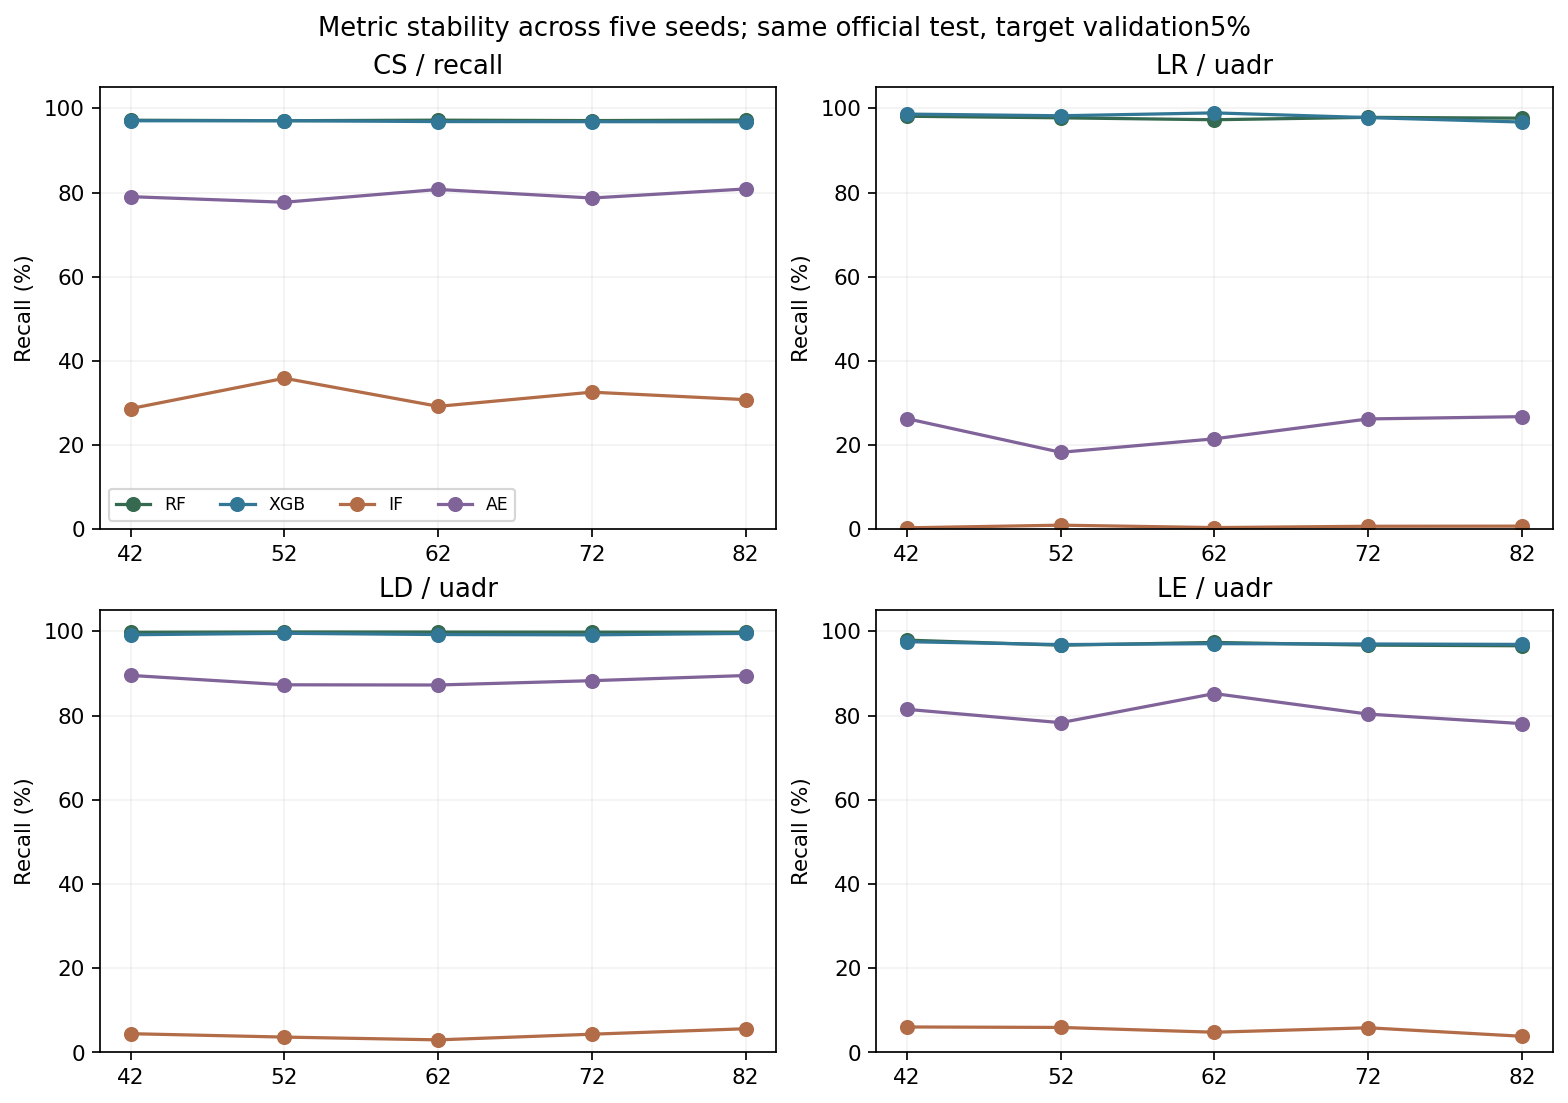
\includegraphics[width=.98\textwidth]{assets/final_diagnostics/SEED_STABILITY.png}
\caption[Độ biến thiên qua năm seed]{Độ biến thiên theo seed trên cùng test. CS dùng recall Attack; LOACO dùng UADR; target validation 5\%.}\end{figure}

\begin{figure}[H]\centering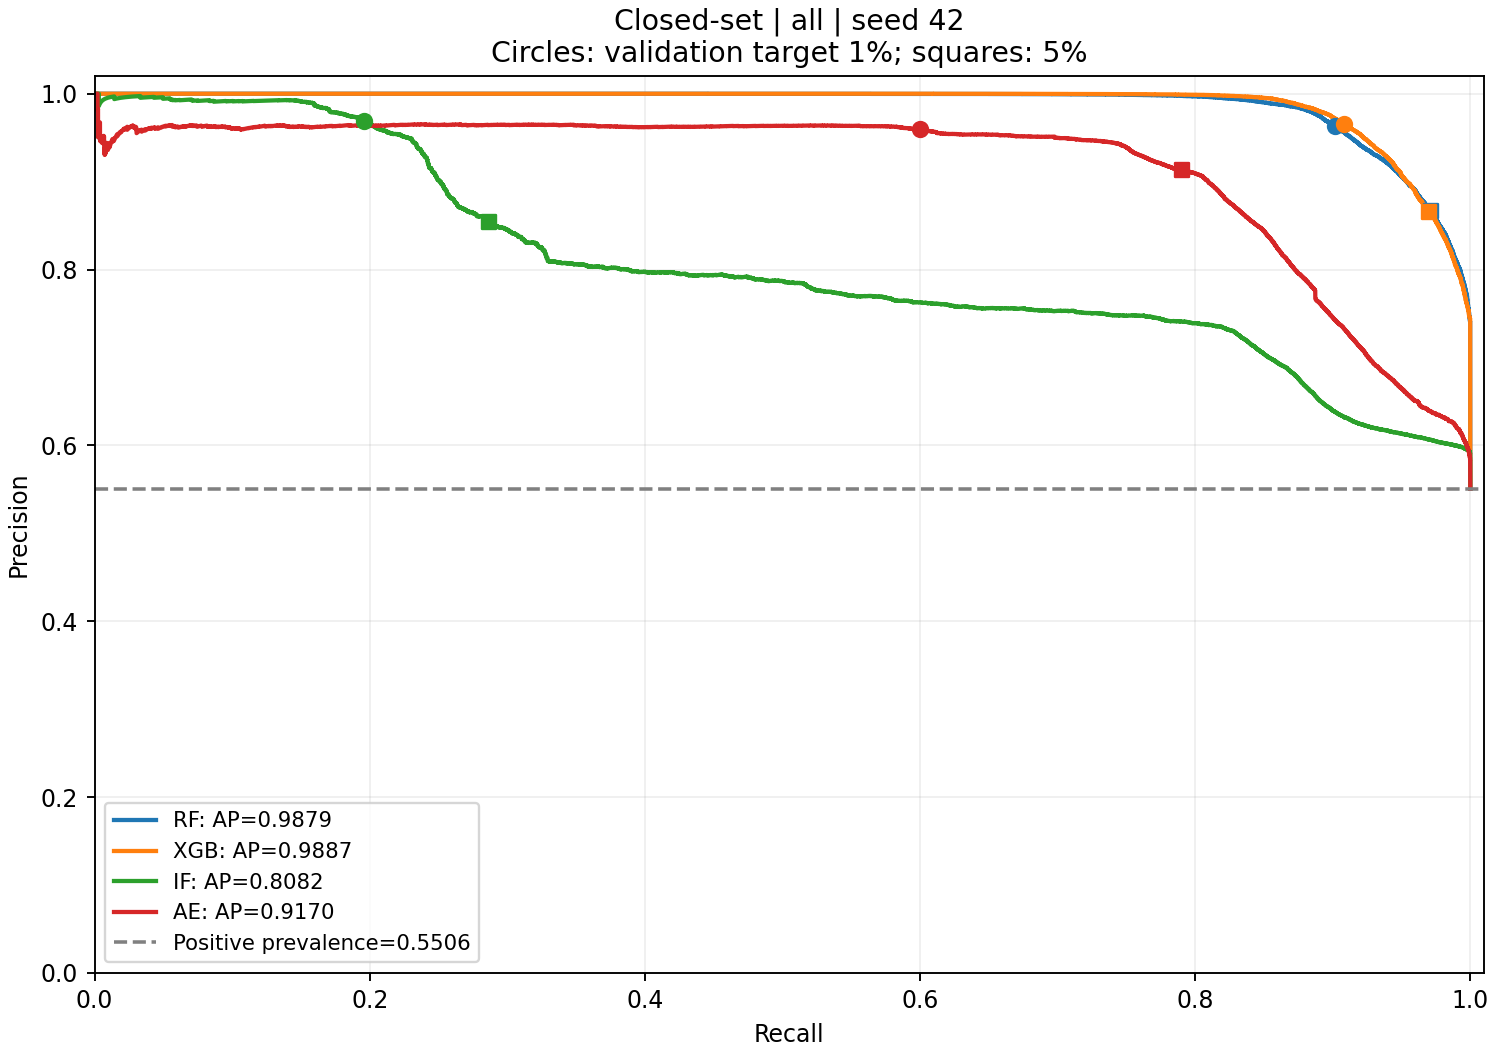
\includegraphics[width=.92\textwidth]{assets/dot3_20261025/PR_CS_all_S42.png}\caption[PR closed-set, seed 42]{PR closed-set cho bốn model, seed 42; AP dùng một score mỗi record, hai target chỉ xác định điểm vận hành.}\end{figure}

\begin{figure}[H]\centering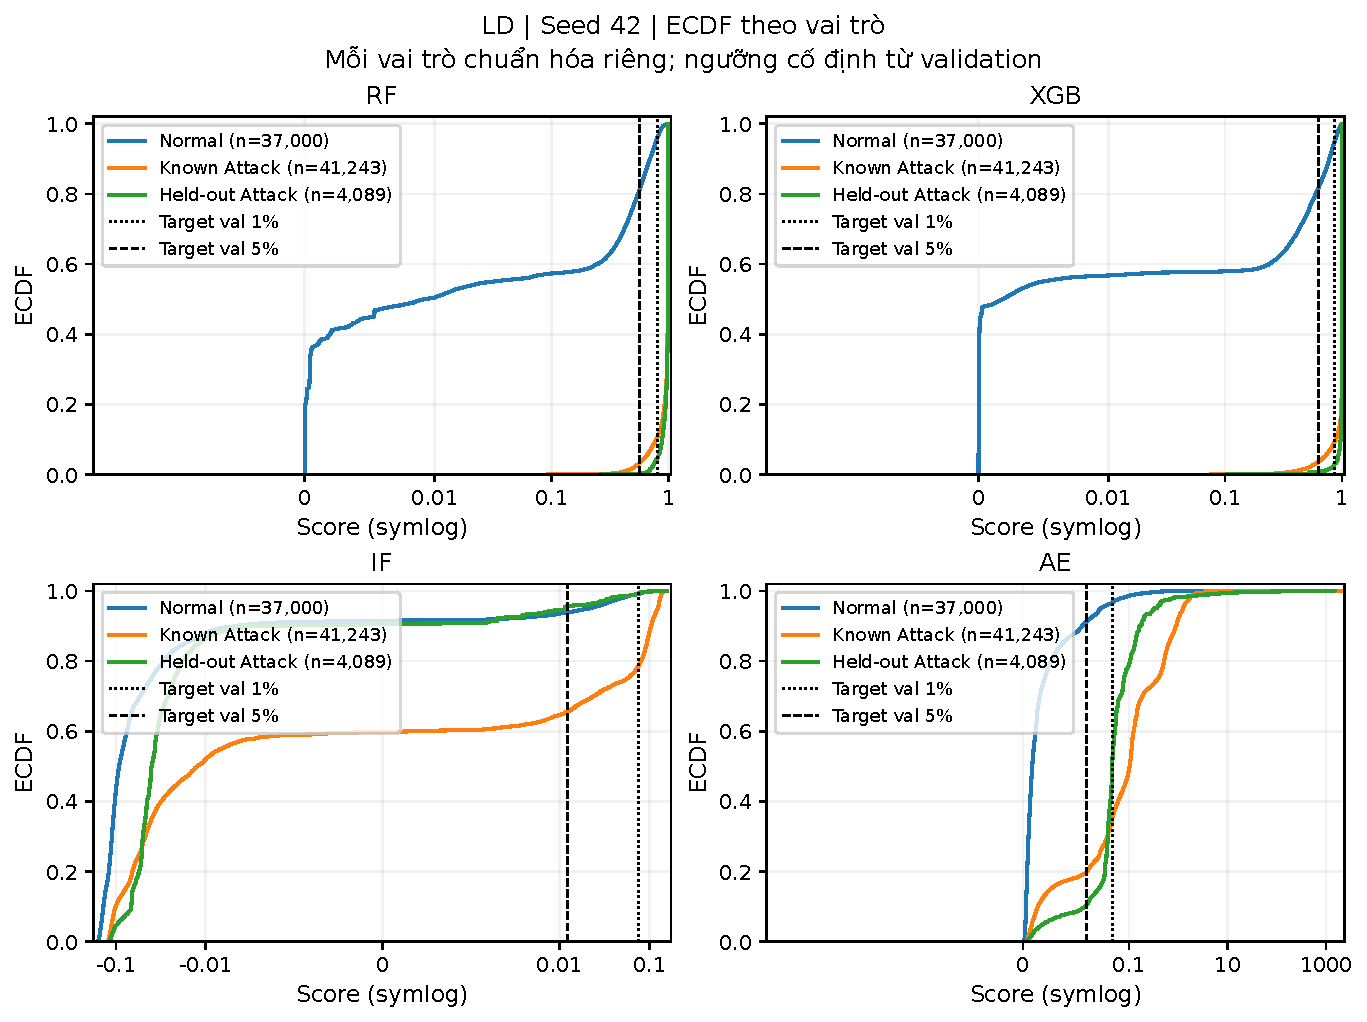
\includegraphics[width=.96\textwidth]{assets/dot3_20261025/SCORE_ECDF_LD_S42.pdf}\caption[ECDF score LOACO DoS]{ECDF score LOACO DoS, seed 42; Normal, known Attack, held-out và hai threshold validation.}\end{figure}

\begin{figure}[H]\centering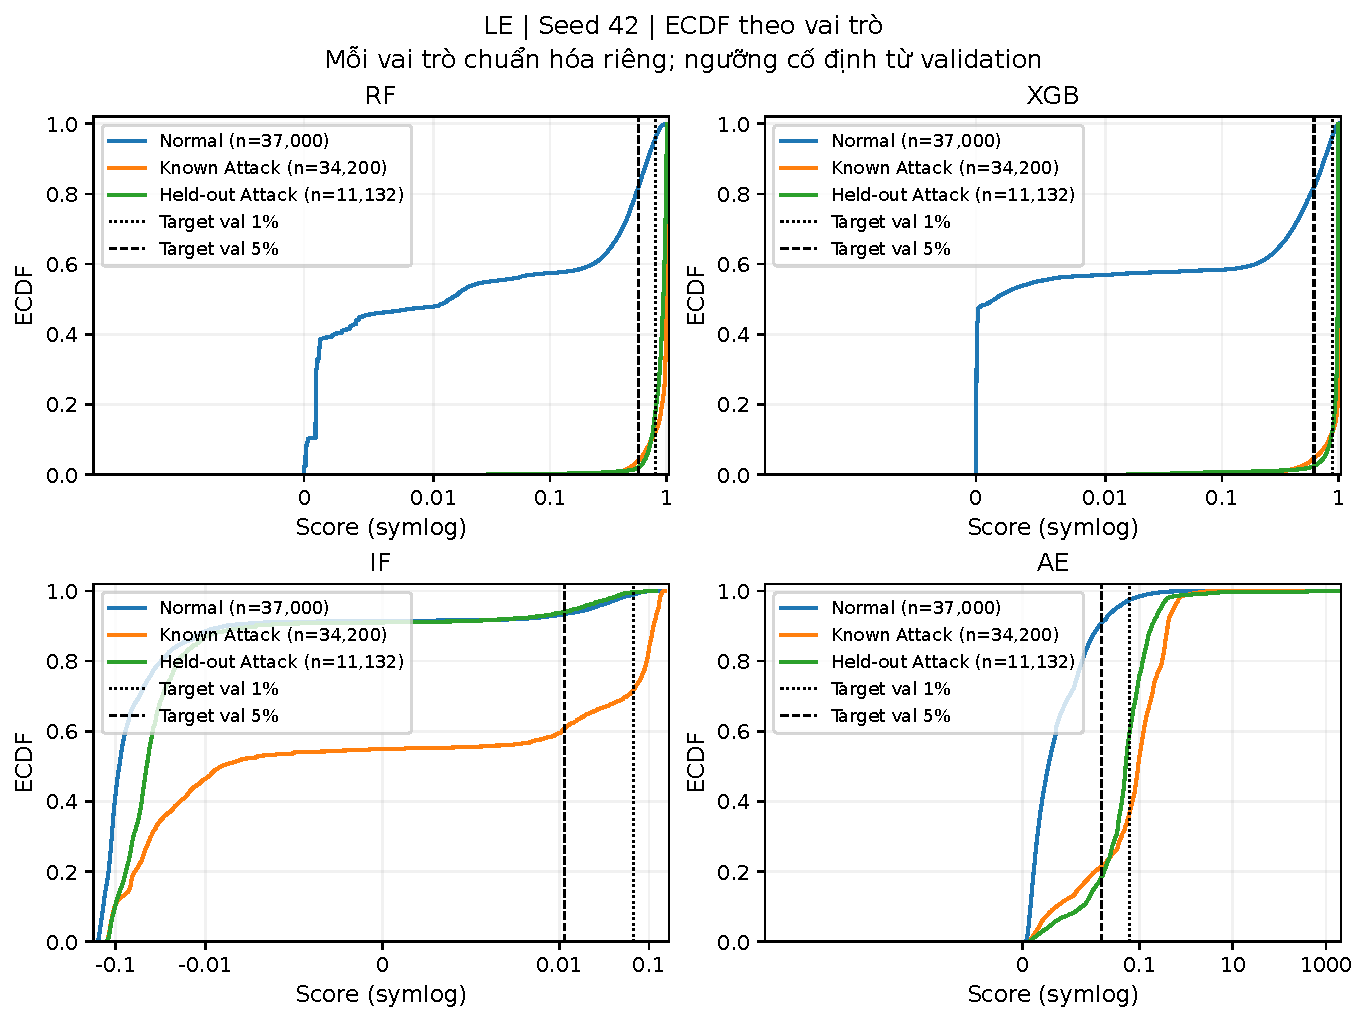
\includegraphics[width=.96\textwidth]{assets/dot3_20261025/SCORE_ECDF_LE_S42.pdf}\caption[ECDF score LOACO Exploits]{ECDF score LOACO Exploits, seed 42; Normal, known Attack, held-out và hai threshold validation.}\end{figure}

\section{Lỗi theo protocol, service và state}
Đặc tả \path{docs/management/DAC_TA_CHAN_DOAN_CUOI_20261025.md} ghi quy tắc trước chạy. Ghép từng prediction về raw official test theo ID, kiểm nhãn/category/role và đủ hai target; 80 run, 13.173.120 dòng prediction và 1.040 metric gốc tiếp tục khớp. Với mỗi giá trị proto/service/state, tính support và TP/FP/TN/FN riêng theo Normal, known Attack, held-out Attack. Ở Normal, tỷ lệ lỗi là FP/support; ở Attack là FN/support. Không cộng ba chiều rồi coi là số record độc lập.

Bảng sau chọn một giá trị có tỷ lệ lỗi mean cao nhất trong mỗi chiều, model và scope, chỉ trong nhóm support ít nhất 100. Hình giữ tối đa sáu nhóm cùng quy tắc. Đây là chọn để thăm dò lỗi trong test đang có, không kiểm định giả thuyết mới, không ước lượng nhân quả, không đại diện nhóm ít mẫu bị lược khỏi hình. CSV giữ toàn bộ nhóm và cả target 1\%/5\%; support của nhóm không thay giữa seed trong cùng role/scenario.
\begingroup\small\setlength{\tabcolsep}{3pt}\renewcommand{\arraystretch}{1.18}
\begin{longtable}{L{.6cm}L{1.1cm}L{1.4cm}L{3.3cm}rL{3.4cm}}
\caption[Lát cắt lỗi theo proto, service, state]{Lát cắt lỗi thăm dò tại target validation 5\%; mean/sample std năm seed; tỷ lệ lỗi theo \%, std theo điểm phần trăm}\\
\toprule Sc. & Model & Chiều & Giá trị & Support & Tỷ lệ lỗi\\\midrule
\endfirsthead
\multicolumn{6}{l}{\small Bảng \thetable\ (tiếp)}\\
\toprule Sc. & Model & Chiều & Giá trị & Support & Tỷ lệ lỗi\\\midrule
\endhead
CS & RF & proto & udp & 8,097 & $25.89\pm0.35$\\
CS & RF & service & ftp & 758 & $32.01\pm2.25$\\
CS & RF & state & INT & 4,485 & $46.65\pm0.54$\\
CS & IF & proto & arp & 987 & $10.15\pm2.66$\\
CS & IF & service & http & 4,013 & $8.45\pm1.15$\\
CS & IF & state & REQ & 1,707 & $33.52\pm3.83$\\
LR & RF & proto & tcp & 1,865 & $3.03\pm0.06$\\
LR & RF & service & - & 2,992 & $2.63\pm0.34$\\
LR & RF & state & FIN & 1,861 & $2.99\pm0.06$\\
LR & IF & proto & udp & 1,304 & $99.95\pm0.04$\\
LR & IF & service & http & 470 & $99.53\pm0.10$\\
LR & IF & state & FIN & 1,861 & $99.88\pm0.02$\\
\bottomrule\end{longtable}\endgroup

\begin{figure}[H]\centering
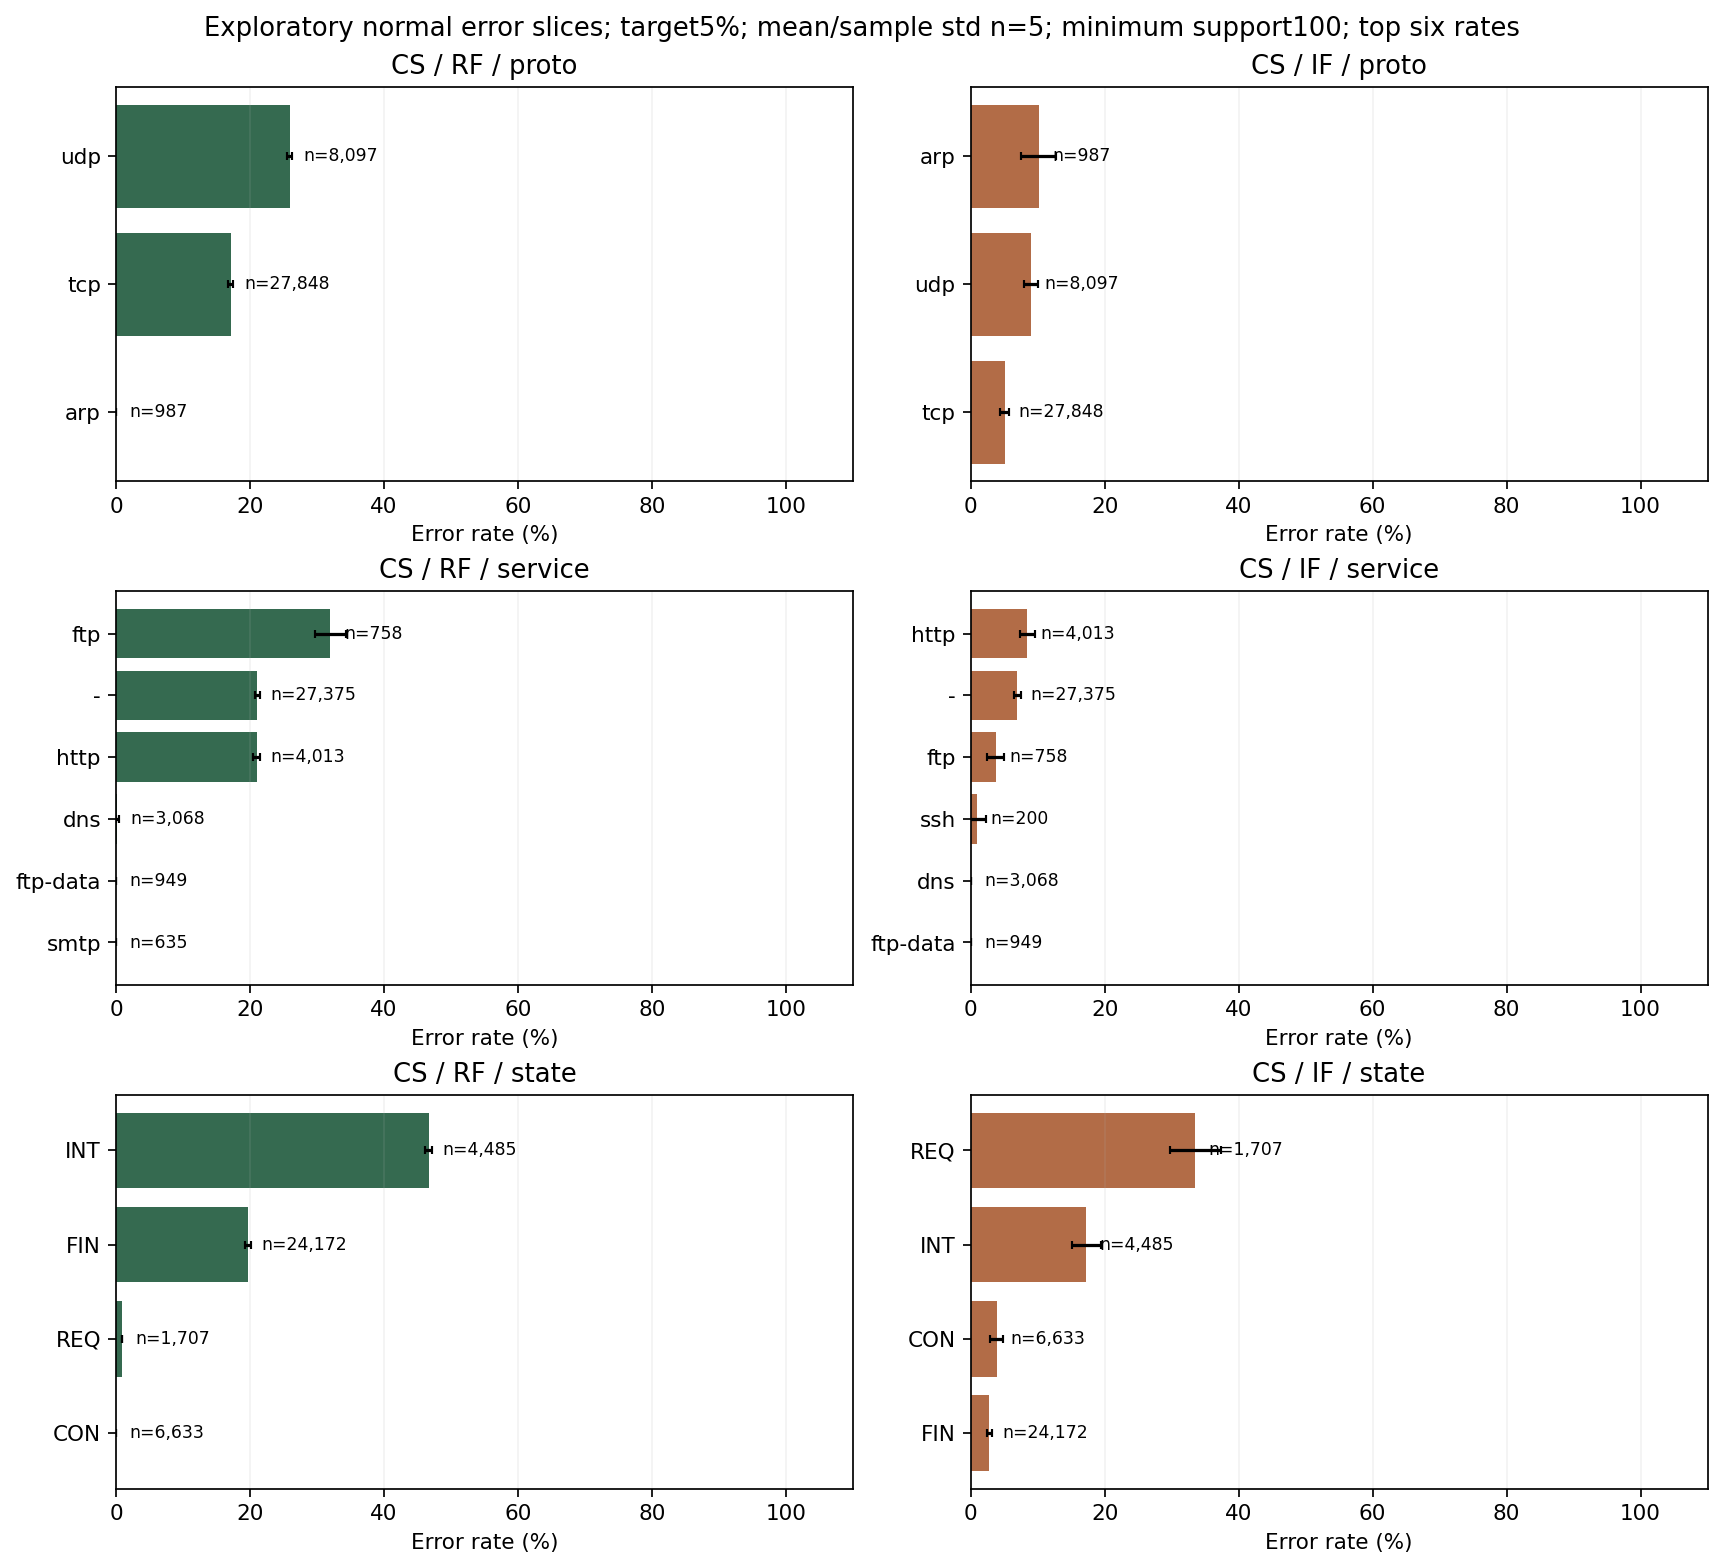
\includegraphics[width=.93\textwidth]{assets/final_diagnostics/FP_GROUPS_CS.png}
\caption[FP theo proto, service, state ở closed-set]{Lỗi Normal closed-set (FP), RF/IF, target validation 5\%; nhóm support tối thiểu 100, chọn tối đa sáu tỷ lệ cao nhất, mean/sample std năm seed.}\end{figure}

\begin{figure}[H]\centering
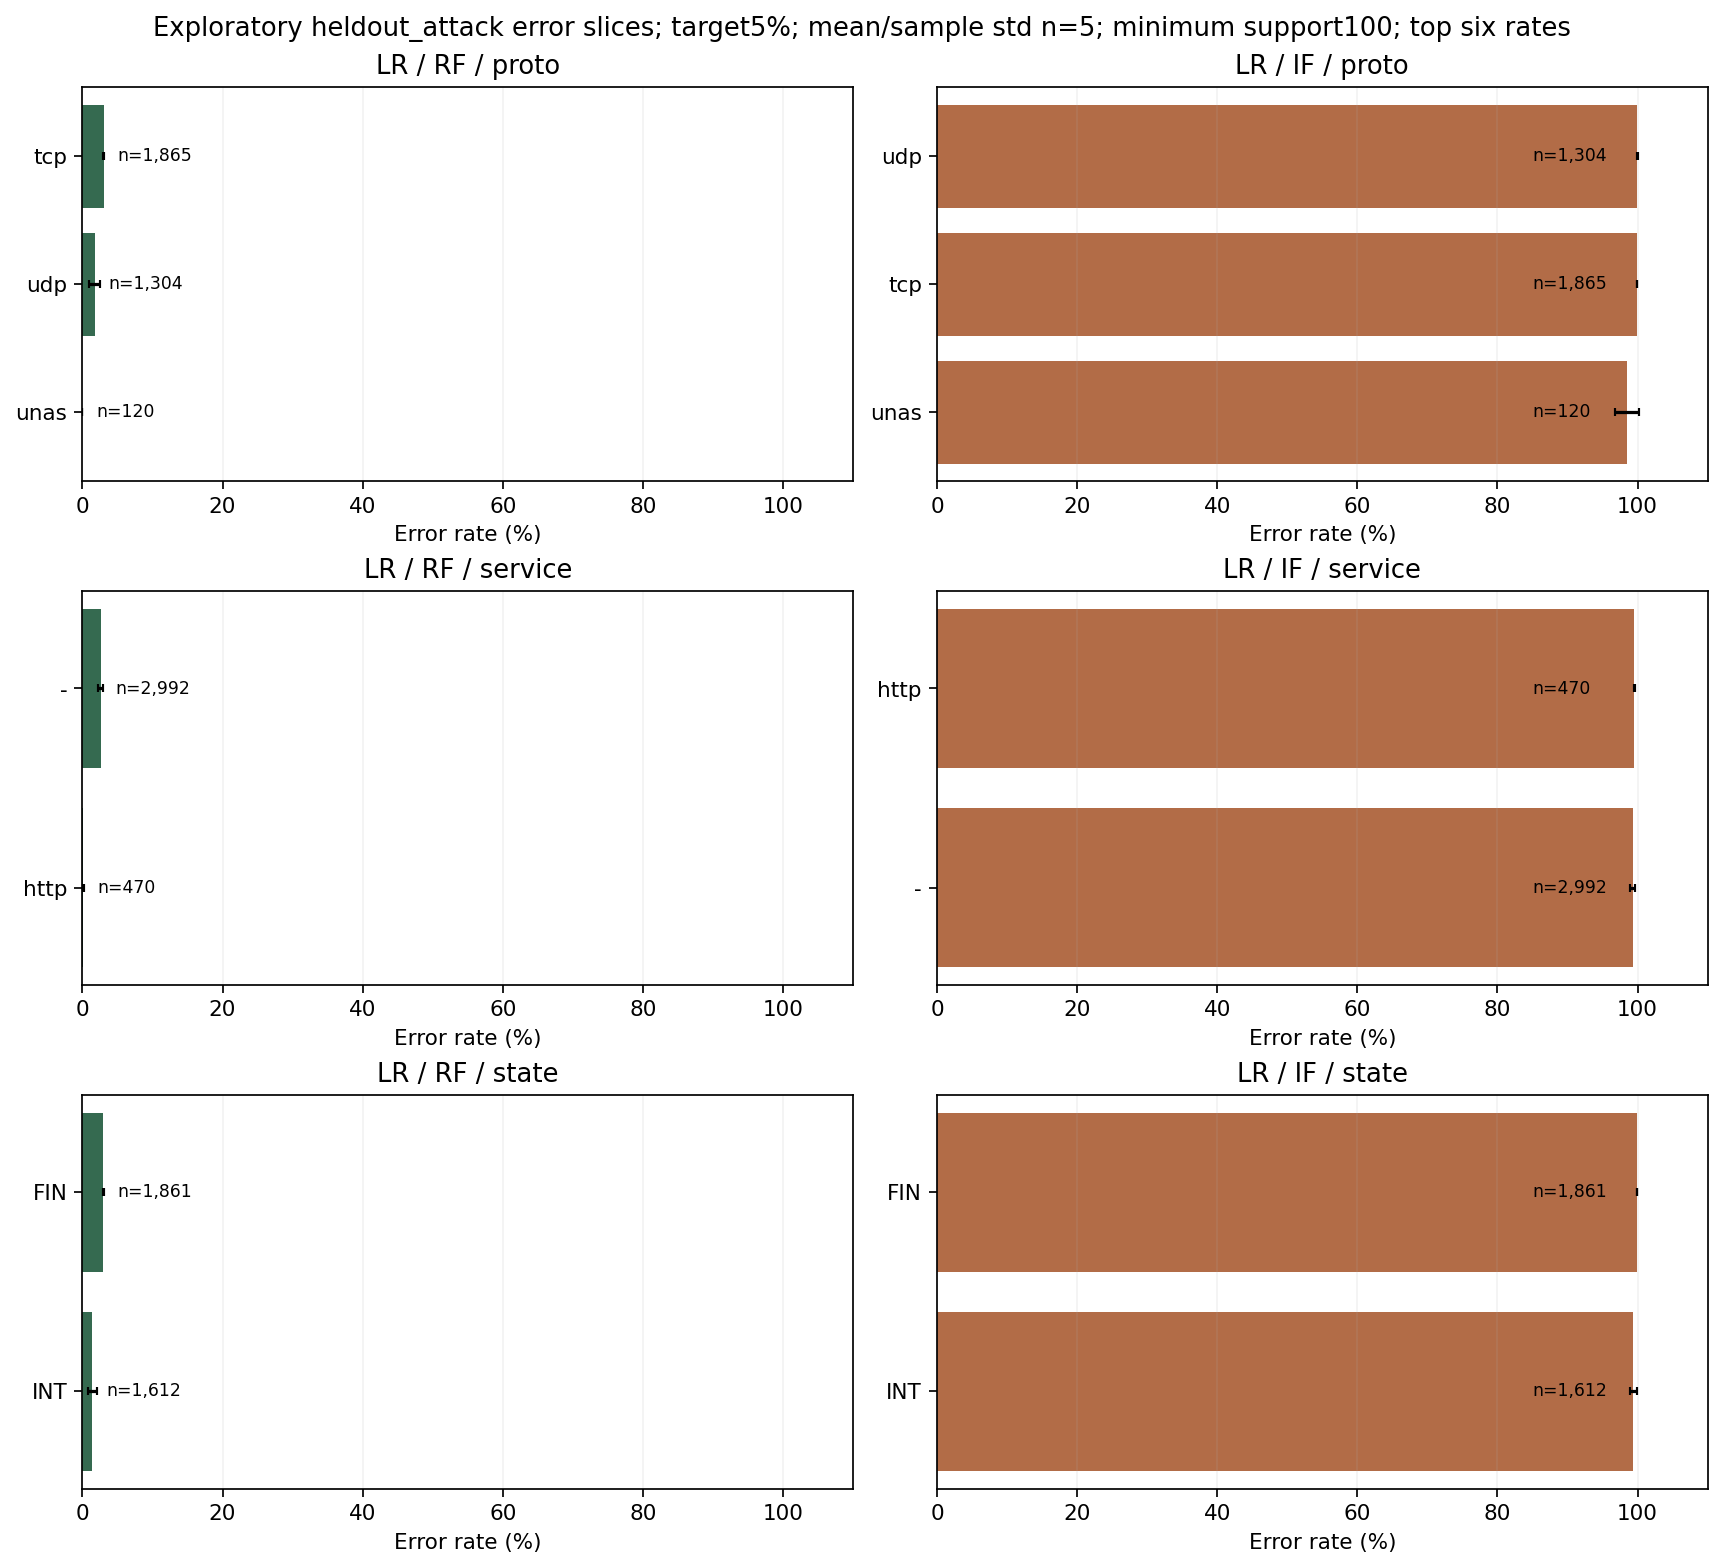
\includegraphics[width=.93\textwidth]{assets/final_diagnostics/FN_GROUPS_LR.png}
\caption[FN theo proto, service, state ở LOACO Reconnaissance]{Lỗi held-out Reconnaissance (FN), RF/IF, target validation 5\%; cùng quy tắc support và chọn nhóm, mean/sample std năm seed.}\end{figure}

Tỷ lệ lỗi cao trong một service/protocol có thể đi kèm loại Attack, phân bố feature và dữ liệu gần giống nhau. Bảng này định vị chỗ cần đọc lại, không chứng minh service hoặc protocol gây lỗi. Khi trao đổi, Thu cần nêu đúng role, giá trị nhóm, support và target trước khi nói phần trăm; Anh kiểm giới hạn của phép ghép và nguồn dữ liệu.

\section{Ví dụ sát ngưỡng, lỗi lặp và bất đồng model}
Mỗi model seed 42, target và role lấy ba record có $|score-threshold|$ nhỏ nhất, hòa thì ID nhỏ trước. Bảng minh họa dưới chỉ lấy record gần nhất ở LR/RF và LR/IF cho Normal/held-out; có cả dự đoán đúng và sai, không chọn riêng trường hợp thuận lợi. dur, sttl, dbytes là feature raw để mở lại dòng gốc. Khoảng cách score chỉ đọc trong cùng model; không so khoảng cách RF với IF để nói model nào tự tin hơn. Feature importance toàn model ở phần trước không giải thích nguyên nhân từng dòng này.
\begingroup\small\setlength{\tabcolsep}{3pt}\renewcommand{\arraystretch}{1.18}
\begin{longtable}{L{1.1cm}rL{.6cm}rL{.9cm}L{1.2cm}rrr}
\caption[Ví dụ dự đoán gần ngưỡng]{Ví dụ gần ngưỡng nhất theo model/vai trò: LR seed 42, target validation 5\%; số học chỉ dùng mô tả}\\
\toprule Model & ID & KQ & $|s-\tau|$ & proto & service & dur (s) & sttl & dbytes\\\midrule
\endfirsthead
\multicolumn{9}{l}{\small Bảng \thetable\ (tiếp)}\\
\toprule Model & ID & KQ & $|s-\tau|$ & proto & service & dur (s) & sttl & dbytes\\\midrule
\endhead
IF & 6577 & FN & 0.00031 & chaos & - & 3e-06 & 254 & 0\\
IF & 75704 & FP & 7.3e-06 & tcp & - & 0.725 & 254 & 612\\
RF & 975 & FN & 0.00032 & tcp & - & 0.639 & 254 & 354\\
RF & 68699 & FP & 1.8e-05 & tcp & - & 0.555 & 254 & 268\\
\bottomrule\end{longtable}\endgroup
\begingroup\small\setlength{\tabcolsep}{3pt}\renewcommand{\arraystretch}{1.18}
\begin{longtable}{L{1cm}L{1.1cm}L{5.2cm}L{5.2cm}}
\caption[Lỗi lặp ở cả năm seed]{Record sai ở cả năm seed tại target validation 5\%; cùng official test; không là năm test độc lập}\\
\toprule Sc. & Model & Normal sai 5/5 / support & Held-out sai 5/5 / support\\\midrule
\endfirsthead
\multicolumn{4}{l}{\small Bảng \thetable\ (tiếp)}\\
\toprule Sc. & Model & Normal sai 5/5 / support & Held-out sai 5/5 / support\\\midrule
\endhead
CS & RF & 5,736 / 37,000 & --\\
CS & XGB & 5,582 / 37,000 & --\\
CS & IF & 1,766 / 37,000 & --\\
CS & AE & 2,390 / 37,000 & --\\
LR & RF & 5,745 / 37,000 & 38 / 3,496\\
LR & XGB & 5,643 / 37,000 & 15 / 3,496\\
LR & IF & 1,684 / 37,000 & 3,459 / 3,496\\
LR & AE & 2,360 / 37,000 & 2,519 / 3,496\\
LD & RF & 5,768 / 37,000 & 6 / 4,089\\
LD & XGB & 5,465 / 37,000 & 10 / 4,089\\
LD & IF & 1,678 / 37,000 & 3,841 / 4,089\\
LD & AE & 2,358 / 37,000 & 339 / 4,089\\
LE & RF & 5,496 / 37,000 & 175 / 11,132\\
LE & XGB & 5,544 / 37,000 & 172 / 11,132\\
LE & IF & 1,651 / 37,000 & 10,299 / 11,132\\
LE & AE & 2,223 / 37,000 & 1,368 / 11,132\\
\bottomrule\end{longtable}\endgroup

CSV \path{ERROR_STABILITY.csv} giữ đủ phân bố sai 0--5 seed cho mỗi role, model, scenario và target. Record sai cả năm seed cho thấy lỗi không biến mất chỉ bằng đổi seed trên test này; không kết luận lỗi bất khả kháng hoặc do một feature cụ thể. Hai model có cùng tỷ lệ tổng vẫn có thể sai ở các record khác nhau. Bảng cặp model ghi số dự đoán khác, số cùng sai và Jaccard của tập lỗi ($|A\cap B|/|A\cup B|$); chưa triển khai ensemble hoặc khẳng định gộp model sẽ tốt hơn.
\begingroup\small\setlength{\tabcolsep}{3pt}\renewcommand{\arraystretch}{1.18}
\begin{longtable}{L{.7cm}L{2.1cm}rrr}
\caption[Bất đồng và giao lỗi giữa model]{Bất đồng và giao lỗi giữa model, seed 42, target validation 5\%, cùng 82.332 record}\\
\toprule Sc. & Cặp model & Khác dự đoán & Cùng sai & Jaccard lỗi\\\midrule
\endfirsthead
\multicolumn{5}{l}{\small Bảng \thetable\ (tiếp)}\\
\toprule Sc. & Cặp model & Khác dự đoán & Cùng sai & Jaccard lỗi\\\midrule
\endhead
CS & RF / XGB & 2,994 & 6,642 & 0.6893\\
CS & RF / IF & 39,380 & 1,622 & 0.0396\\
CS & RF / AE & 16,582 & 2,213 & 0.1177\\
CS & XGB / IF & 39,222 & 1,754 & 0.0428\\
CS & XGB / AE & 16,582 & 2,266 & 0.1202\\
CS & IF / AE & 26,608 & 10,426 & 0.2815\\
LR & RF / XGB & 2,973 & 6,834 & 0.6968\\
LR & RF / IF & 38,738 & 1,703 & 0.0421\\
LR & RF / AE & 15,961 & 2,189 & 0.1206\\
LR & XGB / IF & 38,565 & 1,955 & 0.0482\\
LR & XGB / AE & 16,074 & 2,298 & 0.1251\\
LR & IF / AE & 26,475 & 9,849 & 0.2711\\
\bottomrule\end{longtable}\endgroup

\section{Thời gian, kích thước artifact và phần chưa có bằng chứng lịch sử}
Metadata 80 run có \texttt{duration\_seconds} của toàn run. Không có log tách riêng thời gian train, suy luận cũ hoặc cấu hình phần cứng huấn luyện. Vì vậy cột tổng run dưới đây không được gọi là thời gian train; trường train-only trong CSV để thiếu. Không huấn luyện lại để tạo giả một phép đo lịch sử.

Phép đo mới ngày 25/10 dùng đủ 80 bundle đã lưu, cùng 100 dòng mẫu demo được chọn trước, một lượt warm-up và ba lượt transform+score mỗi bundle. Không gồm load bundle, HTTP, I/O hay khởi động Python. Mean trong bảng là mean qua năm seed của mean ba lượt; std là sample std qua seed; CSV còn giữ std ba lượt từng bundle. Mỗi bundle được đối chiếu score và prediction với dữ liệu khóa, tổng 8.000 score, dung sai $10^{-6}$; không sửa threshold. MB là $10^6$ byte, gồm cả preprocessor và estimator.
\begingroup\small\setlength{\tabcolsep}{3pt}\renewcommand{\arraystretch}{1.18}
\begin{longtable}{L{.6cm}L{1cm}L{3.5cm}L{4.5cm}L{3cm}}
\caption[Thời gian thực thi và kích thước bundle]{Chi phí mô tả, mean/sample std qua năm seed; tổng run lịch sử khác phép đo suy luận hiện tại}\\
\toprule Sc. & Model & Tổng run cũ (s) & Suy luận 100 dòng (ms) & Bundle (MB)\\\midrule
\endfirsthead
\multicolumn{5}{l}{\small Bảng \thetable\ (tiếp)}\\
\toprule Sc. & Model & Tổng run cũ (s) & Suy luận 100 dòng (ms) & Bundle (MB)\\\midrule
\endhead
CS & RF & $20.1260\pm4.4891$ & $1022.2452\pm33.4195$ & $49.8672\pm0.2407$\\
CS & XGB & $8.8732\pm0.3556$ & $84.6965\pm18.5297$ & $0.3884\pm0.0019$\\
CS & IF & $4.5290\pm0.1606$ & $50.0109\pm6.9351$ & $0.7660\pm0.0089$\\
CS & AE & $16.6954\pm3.3233$ & $18.9604\pm7.6687$ & $0.1267\pm0.0009$\\
LR & RF & $19.1338\pm0.7806$ & $822.7703\pm159.3773$ & $48.5958\pm0.1913$\\
LR & XGB & $12.5220\pm1.0736$ & $56.7996\pm8.1157$ & $0.3881\pm0.0072$\\
LR & IF & $6.8108\pm0.4197$ & $53.5590\pm18.8542$ & $0.7658\pm0.0062$\\
LR & AE & $18.3124\pm5.2551$ & $13.3647\pm4.5419$ & $0.1265\pm0.0010$\\
LD & RF & $17.6998\pm0.3891$ & $249.2872\pm62.1727$ & $49.1345\pm0.1507$\\
LD & XGB & $10.3360\pm0.6506$ & $36.4718\pm12.5268$ & $0.3842\pm0.0040$\\
LD & IF & $5.9402\pm0.4465$ & $47.7425\pm13.5185$ & $0.7730\pm0.0054$\\
LD & AE & $20.1788\pm5.1294$ & $11.4271\pm1.7983$ & $0.1256\pm0.0023$\\
LE & RF & $14.0652\pm0.2980$ & $737.9406\pm159.1471$ & $46.1847\pm0.1977$\\
LE & XGB & $8.1334\pm0.2131$ & $142.0197\pm70.3066$ & $0.3861\pm0.0021$\\
LE & IF & $5.3820\pm0.0643$ & $52.9238\pm7.7121$ & $0.7636\pm0.0129$\\
LE & AE & $19.4774\pm2.7479$ & $15.3718\pm5.2217$ & $0.1255\pm0.0008$\\
\bottomrule\end{longtable}\endgroup

Máy dùng đo suy luận ngày 25/10: 12th Gen Intel(R) Core(TM) i5-12450HX, 12 logical CPU, Python 3.14.4; cấu hình hệ điều hành chi tiết ở \path{HARDWARE_CURRENT.json}. Đây là thông tin máy của phép đo ngày 25/10, không xác nhận máy của các run lịch sử. Thời gian trên mẫu nhỏ chịu cache, tải máy và mức song song mặc định; không dùng để kết luận độ trễ live, throughput vận hành hoặc so chi phí train công bằng.

\section{Đối chiếu phạm vi hoàn tất kỹ thuật}
Bộ mới bổ sung các bảng chi phí và chẩn đoán lỗi cùng các hình còn thiếu của kế hoạch. T9 vẫn thiếu bằng chứng thời gian train riêng và phần cứng lịch sử; báo cáo nêu đúng khoảng trống này. Các hình PR closed-set và ECDF từng LOACO, importance đủ scenario nằm trong bộ asset và CSV đi kèm; các hình chính được đưa vào bản đọc. Prototype bản đợt 4 có cùng CSV qua bốn model và giải thích score/feature phù hợp. Các bước này hoàn tất phần chuẩn bị phân tích, không xác nhận việc thành viên đã đọc, tự chạy hoặc giảng viên đã duyệt.

Nguồn chính: \path{docs/evidence/dot_03/final_diagnostics_20261025/}; audit có hash bốn artifact mỗi run, kiểm raw và đối chiếu metric. Nguồn S07 vẫn chỉ sử dụng abstract đã đối chiếu, không viện dẫn kết quả toàn văn chưa đọc. Bản nộp cần cả nhóm xem, sửa, tự giải thích và quyết định dùng nội dung nào.
